\begin{itemize}
\item
\end{itemize}


\section{Introduction}
Nous répondons dans l'ensemble des documents produits par l'hexanôme H4111 à l'appel d'offre lancé par le COPEVUE visant à concevoir un Système de monitoring à distance de sites isolés. Dans ce document sont détaillés avec plus de précisions les constituants  du projet. Nous insisterons donc sur les points de vue organisationnels liés à la conception de notre solution technique.Après avoir resitué le contexte du problème, il s'agira de définir les objectifs ainsi que les contraintes liés à ce type de projet. Sont détaillées aussi dans ce document, les méthodes de travail,la répartition des rôles au sein du groupe d'ingénierie ainsi que le planning de répartition des tâches et des charges de travail. 

\subsection{Présentation du projet}
Le COPEVUE a lancé un appel d'offre dans le cadre de la réalisation d'un système de monitoring de sites isolés. Il s'agit donc de concevoir en premier lieu une solution technique permettant de répondre aux mieux aux exigences fonctionnelles et non fonctionnelles que le COPEVUE formule. De façon synthétique notre équipe va proposer une solution permettant de surveiller des sites naturels difficiles d'accès (souvent à cause des conditions environnementales) et peu peuplés. Dans ces sites isolés sont souvent regroupés des postes de travail et ces zones doivent pouvoir être surveillées en dépit de la distance qui les sépare du bureau de contrôle.

\subsubsection{Contexte du projet}
Notre cas d'étude se limite pour l'instant à considérer une situation simple : comment pouvoir maintenir de manière rentable des réserves de tel ou tel composé à un niveau correct bien que le site de stockage soit situer dans des zones difficiles d'accès ? L'idéal serait donc de pouvoir suivre a distance l'évolution d'un niveau d'un composé en fonction du temps.Le ravitaillement serait ainsi plus raisonnable car on saurait alors la quantité de composant à acheminer sur place. Trouver une solution fonctionnelle à cette problématique permettrait ainsi d'économiser en frais de maintenance mais aussi et surtout d'éviter certaines catastrophe écologique comme par exemple un manque d'eau dans un réservoir lors d'un feu de forêt ou encore une fuite de carburant d'un réservoir de forêt.

\subsubsection{Objectifs du projet}
Les objectifs principaux de ce projet sont pour ainsi dire assez simple conceptuellement parlant, il s'agit en effet de pouvoir surveiller à distance une installation présente sur un site isolé en installant un réseau de capteurs que l'on va pouvoir relevé et maintenir à distance. Dans un deuxième temps, notre sytème permettra de même d'anticiper les pannes et les desagréments au niveau du site à monitorer en générant des alertes au sein d'un site de supervision pouvant être situé à des miliers de kilomètres des sites à surveiller.

\subsubsection{Découpage en phases du projet}
De manière assez classique, la réalisation du système se fera selon le principe de cycle de vie d'un système (cycle en V).
\begin {center}
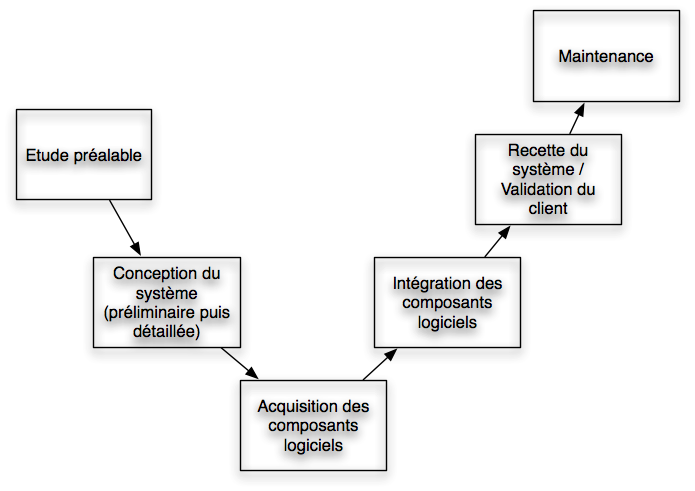
\includegraphics[width=\textwidth]{png/cycleVSysteme.png}
\end {center}

\subsection{Le Plan de Management de Projet}
\subsubsection{Objectifs du PMP}
Ce document a pour objectif de décrire le pilotage de  tout le projet du point de vue du management, c'est à dire l'approche organisationnelle, l'approche produit, l'approche temporelle/charge de travail, les aspects financiers. Il est important de voir que ce dossier ne constitue qu'un draft et qu'ainsi, certaines parties seront volontairement non exhaustives voir incomplètes.

\section{Organisation du projet et différents acteurs}
\subsection{La maitrise d'ouvrage}
La maitrise d'ouvrage sera représentée par la comission européenne COPEVUE en charge de l'envoi de l'appel d'offre aux différents bureaux d'études. Il pourra être intéressant de mettre en oeuvre un site dit tampon ou de référence permettant de tester en temps réel les améliorations apportées au système. Ce système pourra être testé en présence de représentants du
 COPEVUE pour attester de l'avancée du travail.
\subsection{La maitrise d'oeuvre}
L'équipe de travail en charge de ce projet sera augmentée de quelques personnes par rapport à l'équipe en charge de la réponse à l'appel d'offre.
Notre groupe se compose donc au final de :

\begin{itemize}
\item Le Chef de projet.
\item Le Responsable qualité.
\item Le Responsable du déploiement du système.
\item Le Responsable du pôle R\&D.
\item Une équipe commerciale.
\end{itemize}
Le pôle R\&D étant constitué d'ingénieur chargé de maintenir le système mais aussi de le faire évoluer.
Le Responsable du déploiement est quant à lui chargé de manager les techniciens qui intègrent le système mais aussi de reporter les éventuels bugs d'intégration à l'équipe R\&D.

\subsection{Documents de références}
\begin{itemize}
\item Aide à la rédaction d'une procédure
\item Dossier d'initialisation
\item Procédure de décomposition d'un système en sous-systèmes et sous projets
\end{itemize}

\section{Démarche de développement du système}
D'après le cycle de vie du système décrit plus haut, il est nécessaire de se rendre compte qu'il faut découper le système en briques élémentaire avant tout début de travail de réalisation. Le système complexe doit donc être réparti en différents sous système qui eux mêmes donneront lieu à la rédaction de plusieurs cahiers des charges. Les cahiers des charges ne doivent pas se limiter aux parties logicielles mais doivent prendre en compte de même les projet matériels, d'intégration, de formation de l'équipe de maîtrise d'oeuvre.

\subsection{Rappel de la méthode de découpage d'un système en sous système}

\begin {center}
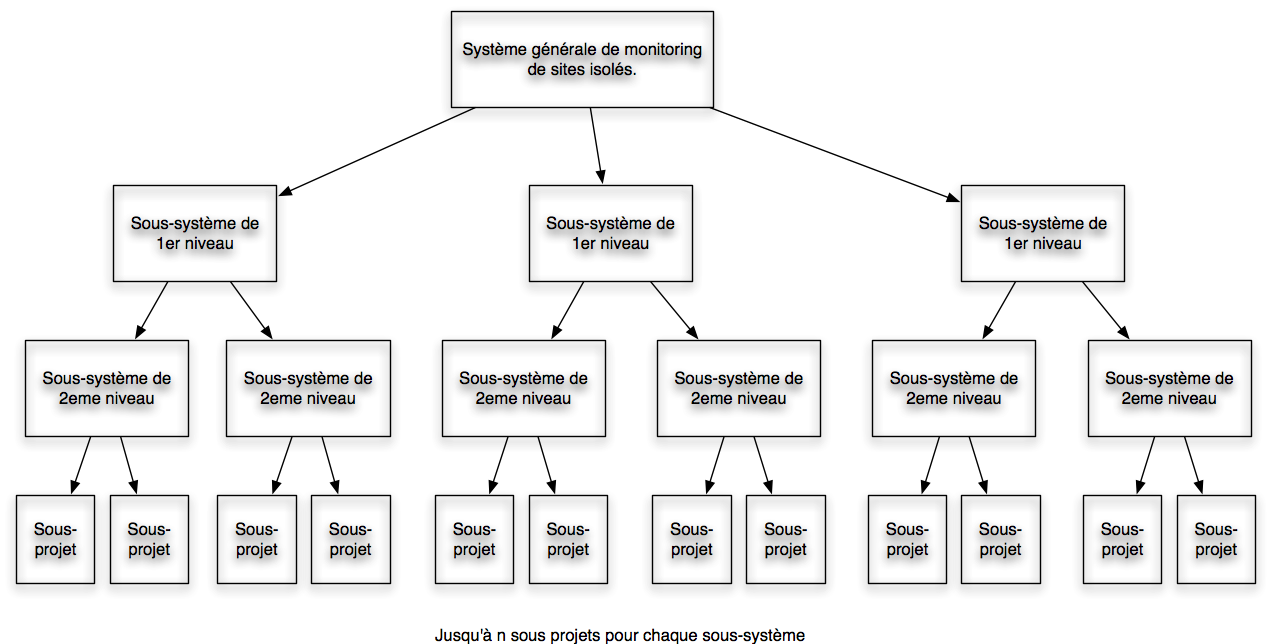
\includegraphics[width=\textwidth]{png/decoupageType.png}
\end {center}


\subsection{Découpage du système monitoring de sites isolés}
\subsubsection{Découpage du système en sous-systèmes}
\subsubsection{Identification des projets et sous-projets}
\subsection{Description des sous-projet}
\subsubsection{Choix des projets retenus pour établissement cahier des charges}

\section{Moyens à mettre en oeuvre}
\subsection{Moyens matériels}
\subsection{Moyens logiciels}
\subsection{Moyens humains}
\subsubsection{Evaluation des charges de travail}

\section{Principes d'actions sur le système à distance}
\subsection{Configuration à distance du système}
\subsection{Maintenance à distance du système}
\section{Conclusion}






